\subsection{UC9 - Salvataggio visualizzazione}
    \label{uc9}
    
    \begin{figure}[htbp]
        \centering
        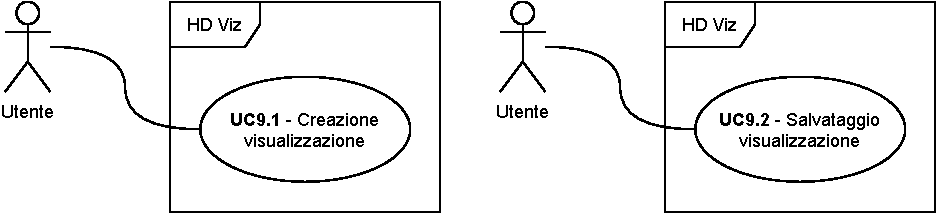
\includegraphics[width=0.9\textwidth]{source/sections/casi-uso/diagrams/uc9.pdf}
        \caption{UC9 - Salvataggio visualizzazione}
        \label{fig:uc9}
    \end{figure}


    \begin{itemize}
    \item \textbf{Attore}: utente;
    \item \textbf{Descrizione}: l'utente salva la visualizzazione;
    \item \textbf{Precondizione}: 
    \begin{itemize}
        \item eseguito l'upload del dataset come matrice $N\times M$ (\hyperref[uc1]{UC1});
        \item selezionato un tipo di visualizzazione (\hyperref[uc2]{UC2});
        \item dati elaborati (\hyperref[uc8]{UC8});
        \item visualizzazione creata (\hyperref[uc9.1]{UC9.1}).
    \end{itemize}  
    \item \textbf{Postcondizione}: l'utente ha salvato la visualizzazione come file immagine PNG;
    \item \textbf{Output}: file PNG con la visualizzazione richiesta;
    \item \textbf{Scenario Principale}: 
    \begin{enumerate}
        \item l'utente carica il suo dataset (\hyperref[uc1]{UC1});
        \item l'utente seleziona il tipo di visualizzazione tra quelle disponibili (\hyperref[uc2]{UC2});
        \item l'applicazione elabora i dati (\hyperref[uc8]{UC8});
        \item l'applicazione crea la visualizzazione;
        \item l'utente salva (cliccando sul pulsante salva) la visualizzazione in formato PNG.
    \end{enumerate}
    \end{itemize}